\documentclass[border=10pt]{standalone}
\usepackage{amsmath,amssymb}
\usepackage{pgfplots}
\pgfplotsset{compat=1.18}
\usetikzlibrary{arrows.meta}

\begin{document}
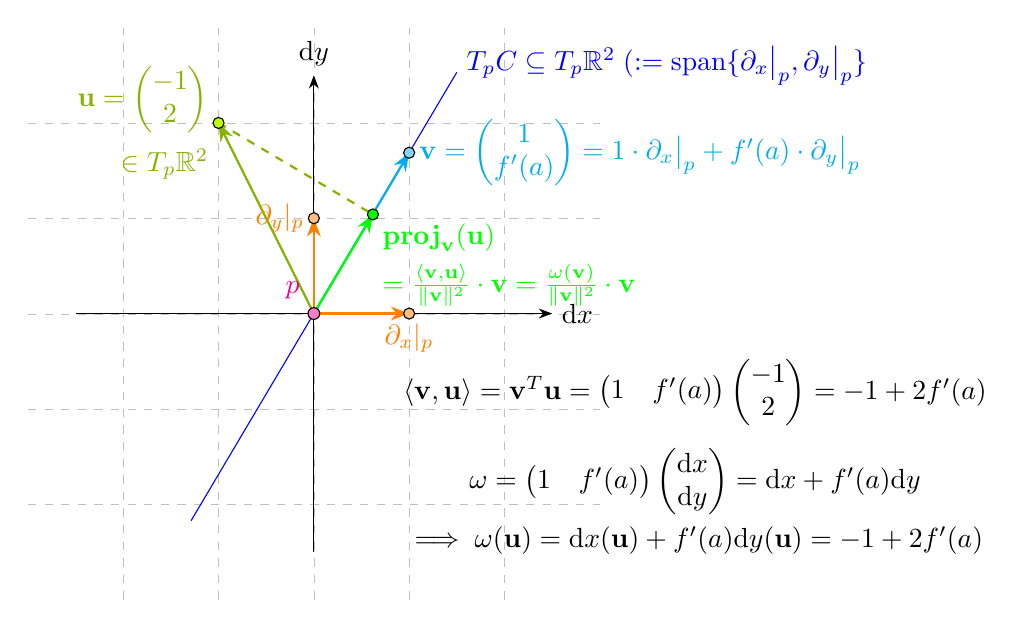
\begin{tikzpicture}
% --- Pre-calculate all values for the new function ---
\pgfmathsetmacro{\a}{2.25}              % x-coordinate of point p
\pgfmathsetmacro{\ay}{\a^3-3*\a^2+5} % y-coordinate using the new function
\pgfmathsetmacro{\slope}{3*\a^2 -6*\a} % Slope using the new derivative

\pgfmathsetmacro{\dx}{1}             % Vector x-component (made slightly smaller for visibility)
\pgfmathsetmacro{\dy}{\slope * \dx}   % Vector y-component
\pgfmathsetmacro{\endx}{\a + \dx}     % Vector end-point x
\pgfmathsetmacro{\endy}{\ay + \dy}     % Vector end-point y

% --- Pre-calculate label position for the tangent line ---
\pgfmathsetmacro{\labelx}{\a + 0.5}
\pgfmathsetmacro{\labely}{\ay + \slope*(\labelx-\a)}
\begin{axis}[
	axis lines=center,
	axis line style={opacity=0},
	%	xlabel=$\mathrm{d}x$,ylabel=$\mathrm{d}y$,
	xtick=\empty,ytick=\empty,
	legend pos=north west,
%	xmin=-2.5, xmax=5,   % Adjusted axis limits
%	ymin=-1, ymax=6,    % Adjusted axis limits
	restrict y to domain=-1:6,
	axis equal, % Ensures slopes are visually correct
	clip=false,
	]
	\pgfplotsextra{
		\pgfmathsetmacro{\xcenter}{2.25}
		\pgfmathsetmacro{\ycenter}{1.2}
		\pgfmathsetmacro{\xstep}{1}
		\pgfmathsetmacro{\ystep}{1}
		\pgfmathsetmacro{\xcount}{6} % total grid width = xcount * xstep
		\pgfmathsetmacro{\ycount}{6}
		
		\foreach \i in {-2,-1,0,1,2} {
			\pgfmathparse{\ycenter + \i*\ystep}
			\edef\yy{\pgfmathresult}
			\draw[lightgray, very thin, dashed]
			(axis cs:{\xcenter - \xcount*\xstep/2}, \yy)
			-- (axis cs:{\xcenter + \xcount*\xstep/2}, \yy);
		}
		\foreach \j in {-2,-1,0,1,2} {
			\pgfmathparse{\xcenter + \j*\xstep}
			\edef\xx{\pgfmathresult}
			\draw[lightgray, very thin, dashed]
			(axis cs:\xx, {\ycenter - \ycount*\ystep/2})
			-- (axis cs:\xx, {\ycenter + \ycount*\ystep/2});
		}
	}


	\draw[-Stealth] (\a-2.5,\ay) to (\a+2.5,\ay) node[right] {$\mathrm{d}x$};
	\draw[-Stealth] (\a,\ay-2.5) to (\a,\ay+2.5) node[above] {$\mathrm{d}y$};

	% --- Draw the tangent vector v ---
	\addplot[domain=-2:3.75, samples=100, blue] {\ay + \slope*(x-\a)};
	\node[right, blue] at (axis cs:3.75, 3.8) {$T_pC\subseteq T_p\mathbb{R}^2\; (:=\mathrm{span}\{\partial_x\big|_p,\partial_y\big|_p\}$};
	\draw[
	-{Stealth},
	thick,
	cyan,
	] (axis cs: \a, \ay) -- (axis cs: \endx, \endy)
	node[right] {$\mathbf{v}=\begin{pmatrix} 1\\ f'(a) \end{pmatrix}=1\cdot\partial_x\big|_p+f'(a)\cdot \partial_y\big|_p$};
	\draw[
	-{Stealth},
	thick,
	lime!70!black,
	align=center,
	] (axis cs: \a, \ay) -- (axis cs: \a-1, \ay+2)
	node[left, align=right] {$\mathbf{u}=\begin{pmatrix} -1\\ 2 \end{pmatrix}$\\[5pt]$\in T_p\mathbb{R}^2$ 
%		$=(-1)\cdot\partial_x\big|_p+2\cdot \partial_y\big|_p$
	};
%	
	\draw[-Stealth,thick,orange] (\a,\ay) to (\a+1,\ay);
	\draw[-Stealth,thick,orange] (\a,\ay) to (\a,\ay+1);
%	\draw[gray!50, dashed] (\a-4,\ay-4) grid (\a+4,\ay+4);
%	\draw[fill=orange!50] (\a+1,\ay) circle (1.5pt) node[below, orange, align=center, font=\scriptsize] {$\begin{pmatrix}
%			1\\ 0
%		\end{pmatrix}_p$\\[5pt] $=\frac{\partial}{\partial x}\big|_p=\partial_x\big|_p$};
%	\draw[fill=orange!50] (\a,\ay+1) circle (1.5pt) node[left, orange, align=right, font=\scriptsize] {$\begin{pmatrix}
%			0\\ 1
%		\end{pmatrix}_p$\\[5pt] $=\frac{\partial}{\partial y}\big|_p=\partial_y\big|_p$};
%	\draw[fill=cyan!50] (\a+\dx, \ay+\slope) circle (2pt);
	
	% --- Mark the point p ---
	\draw[fill=cyan!50] (\endx,\endy) circle (2pt);
	\draw[fill=orange!50] (\a+1,\ay) circle (2pt) node[below, orange] {$\partial_x|_p$};
	\draw[fill=orange!50] (\a,\ay+1) circle (2pt) node[left, orange] {$\partial_y|_p$};
	\draw[lime!70!black, thick, dashed] (\a-1,\ay+2) to (\a+0.62,\ay+1.04);
	\draw[-Stealth, green, thick] (\a,\ay) to (\a+0.62,\ay+1.04);
	\draw[fill=lime] (\a-1,\ay+2) circle (2pt);
	\draw[fill=green] (\a+0.62,\ay+1.04) circle (2pt) node[below right, green, align=left] {$\mathbf{proj}_{\mathbf{v}}(\mathbf{u})$\\ [3.5pt] $=\frac{\langle\mathbf{v},\mathbf{u}\rangle}{\|\mathbf{v}\|^2}\cdot\mathbf{v}=\frac{\omega(\mathbf{v})}{\|\mathbf{v}\|^2}\cdot\mathbf{v}$};
	
	\node[circle, fill=magenta!50, draw=black, inner sep=1.5pt, label={above left:$\color{magenta}p$}] at (axis cs: \a, \ay) {};
	
	\node[align=center] at (axis cs: \a+4, \ay-1.5) {$\langle\mathbf{v},\mathbf{u}\rangle=\mathbf{v}^T\mathbf{u}=\begin{pmatrix}
		1& f'(a)
	\end{pmatrix}\begin{pmatrix}
		-1 \\ 2
	\end{pmatrix}=-1+ 2f'(a)$\\ [7.5pt]
	$\omega=\begin{pmatrix}
		1 & f'(a)
	\end{pmatrix}\begin{pmatrix}
		\mathrm{d}x \\ \mathrm{d}y
	\end{pmatrix}=\mathrm{d}x+f'(a)\mathrm{d}y$\\ [3pt]
	$\implies\omega(\mathbf{u})=\mathrm{d}x(\mathbf{u})+f'(a)\mathrm{d}y(\mathbf{u})=-1+2f'(a)$
	};
\end{axis}
\end{tikzpicture}
\end{document}